\setcounter{equation}{0}

\chapter{Systems and Exploitation}

\section*{Introduction}
The following chapter is an introduction to case studies of well knowns exploits, intoducing mobile systems and gaming consoles ( The easiest to hack, for their exploitation is mainstream). This is an introduction to the basics of actual life exploiting and will go into details on how the exploits were used, how to install them, their working and also how to replicate it. Specific systems will be covered in a one to one case based scenario. 

\section*{Terminology}
There are some very common terms encountered while browsing through this piece and also while refering to external resources specific to console exploitation (As I told you, it \textit{was} (is) very mainstream). Exploitation of systems with only a software is known as a softmod, whereas one done by physically modifying your hardware is known as hardmod. There are obvious advantages to both, a softmod is usually protected from in the next firmware update whereas hardmods are usually based on hardware vulnerabilities (But not always) and thus are harder to protect against after product is in the hands of the public.

\section{PSP}
One of the most exploited (\textit{Hacked}) system out there. It is the one that even I have reaped the benifits of, by doing \textit{legal} things, of course. It is also the one which I remember following to check out if the next version was exploitable, was it safe, did the risks outweigh the positives, etc. So here, I will explain how the PSP was exploited, why was it \textit{easy} and also replication.

\section{Android}
For android devices, it is not technically exploitaion as Android does not dissalow it, it is the OEMs which refuse access to root for customers. So rooting \textit{technically}, if the OEM ( like Xiaomi ) allows it, is not exploitaiton, but it does allow access to the complete system, so I am going to proceed with calling it exploitaiton of Android Rooting on android differs from phone to phone ( Or more like OEMs to OEMs ), and can be trivially easy or a fairly complicated process. But the general flow of work goes like this: Normal Device $\rightarrow$ Unlocking Bootloader $\rightarrow$ Installing a custom recovery $\rightarrow$ Installing a root manager ( Like magisk or SuperSU ) $\rightarrow$ Reboot $\rightarrow$ Rooted Android 

\subsection{Bootloader}
The bootloader in an android device is hidden and is not accessible to the normal user. It is locked by the OEM, so in order to access it, it has to be unlocked first. The method differs for every phone, and the details can be found on XDA Developers website\footnote[1]{xda-developers.com}. Bootloader is explained in detail in the Operating System section, but a brief understanding is that it is piece of code that points which OS ( More specifically the kernel\footnote[2]{Learn More} ) to load. So the bootloader, after being unlocked will allow us to load a custom OS ( Known as recovery ). This is a standalone OS which allows us to \textit{flash} a zip to the main partition.

\subsubsection{Unlocking the Bootloader}
TO DO

\begin{figure}
    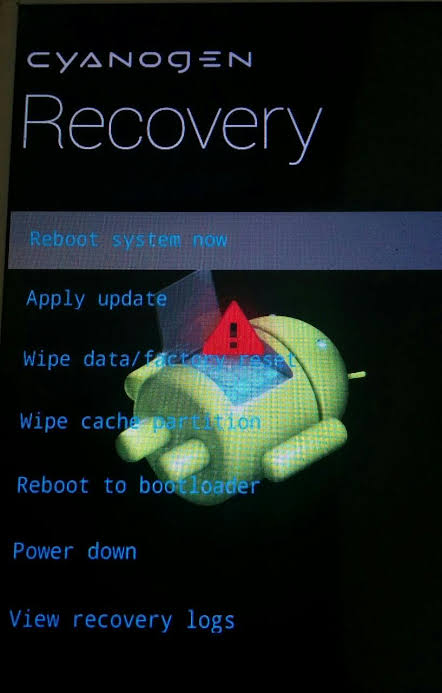
\includegraphics[width = 0.50\textwidth, center]{gfx/recovry.jpeg}    
    \caption{Recovery}
\end{figure}

\subsection{Recovery}
Recovery is an OS, which has a single purpose of allowing recovery. What it means is that it is a small OS which helps in fixing your main OS by providing tools to fix it ( Kind of like the live linux systems ). It is a minimal shell which allows for some fastboot and posix commands to run. It is most usefull in flashing zips which are either ROMs, custom kernels, or root binaries.The vanilla recovery that comes with the device does not allow for any such modifications, and this is where a custom recovery comes into picture. It allows for any modification and installation from within the recovery itself.

\subsubsection{Custom Recovery}
Custom recovery is the software which performs function of a recovery but allows for remote application i.e no need for another device to give commands to the system for it to work. One of the earlier custom recovery software was ClockworkMod which was one of the primary custom recovery for Android versions till 4.0, after which TWRP started to take over as the preferred recovery software.

\subsection{ADB and Fastboot}
ADB and Fastboot are utilities 

\subsubsection{Andoid Debugging Bridge}
Android Debugging Bridge ( known as ADB ) is a tool which allow for 
communication with an android device via USB. It is a shell with basic 
commands that allow a device to execute \textit{debug} commands. It is 
a basic version of a UNIX shell.

\begin{figure}
    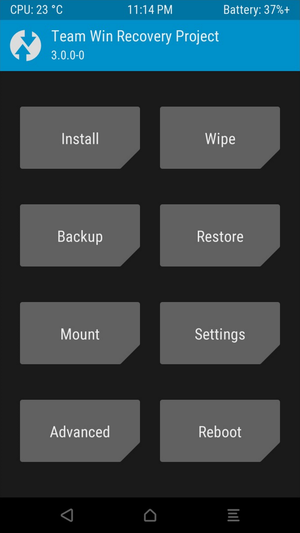
\includegraphics[width = 0.50\textwidth, center]{gfx/twrp.png}    
    \caption{TWRP}
\end{figure}